\documentclass{cours}

\let\oldfrac\frac
\let\frac\tfrac % lazy inline style in trig functions

\title{Complément sur la Trigonométrie}

\begin{document}
    \maketitle{19}

    \begin{Gpartie}{Rappels}
        $\forall x\in\mathbb{R},~
        \begin{aligned}[t]&\cos\,\left(\frac{\pi}{2}-x\right)=\sin\,(x) \\
            &\sin\,\left(\frac{\pi}{2}-x\right)=\cos\,(x) \\
            &\cos^2(x)+\sin^2(x)=1 \\
            &\sin\,(x)=-\sin\,(-x) \\
            &\cos\,(x)=\cos\,(-x)
        \end{aligned}$
    \end{Gpartie}

    \begin{Gpartie}{Formules d'Addition et Duplication} 
        \begin{Spartie}{Formule d'Addition} 
            \begin{center}
                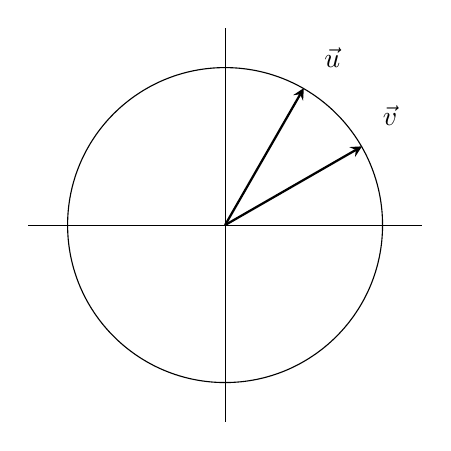
\begin{tikzpicture}[scale=2]
                    \draw (0,0) coordinate (o) circle (1);
                    \draw (-1.25,0) -- (1.25,0) coordinate (a);
                    \draw (0,-1.25) -- (0,1.25);
                    \coordinate (u) at (0.5,0.87);
                    \coordinate (v) at (0.87,0.5);
                    \draw[-stealth, thick] (0,0) -- (u) node[label=above right:$\vec{u}$] {};
                    \draw[-stealth, thick] (0,0) -- (v) node[label=above right:$\vec{v}$] {};
                    % \draw pic["$a$", draw=orange, <->, angle eccentricity=1.2, angle radius=0.75cm]{angle=a--o--u};
                \end{tikzpicture}
                \parbox{\linewidth}{\captionof{figure}{\centering Représentation de $\vec{u}$ et $\vec{v}$ dans le Cercle Trigonométrique}}
                $\lvert\lvert\vec{u}\rvert\rvert=\lvert\lvert\vec{v}\rvert\rvert=1\quad\left(\overrightarrow{OI}\,;\vec{u}\right)=a\quad\left(\overrightarrow{OI}\,;\vec{v}\right)=b\quad\vec{u}\begin{psmallmatrix}\cos a \\ \sin a\end{psmallmatrix}\quad\vec{v}\begin{psmallmatrix}\cos a \\ \sin a\end{psmallmatrix}$
            \end{center}

            Or, $\vec{u}\cdot\vec{v}=\cos\,(a)\cos\,(b)+\sin\,(a)\sin\,(b)$
            
            Mais, $\vec{u}\cdot\vec{v}=\lvert\lvert\vec{u}\rvert\rvert\times\lvert\lvert\vec{v}\rvert\rvert\times\cos\,(\vec{u}\,; \vec{v})\quad$ avec $(\vec{u}\,; \vec{v})=a-b$ ou $b-a$ 

            Ainsi : \[\cos\,(a-b)=\cos\,(a)\cos\,(b)+\sin\,(a)\sin\,(b)\]
            \begin{SSpartie}{Exemple} 
                $\begin{aligned}[t]
                    \cos\,\left(\frac{\pi}{12}\right)=\cos\,\left(\frac{\pi}{3}-\frac{\pi}{4}\right) &= \cos\,\left(\frac{\pi}{3}\right)\cos\,\left(\frac{\pi}{4}\right)+\sin\,\left(\frac{\pi}{3}\right)\sin\,\left(\frac{\pi}{4}\right) \\
                    &= \dfrac{1}{2}\times\dfrac{\sqrt{2}}{2}+\dfrac{\sqrt{3}}{2}\times\dfrac{\sqrt{2}}{2} \\
                    &= \dfrac{\sqrt{2}+\sqrt{6}}{4}
                \end{aligned}$
            \end{SSpartie}
            Autres Formules :
            \[\cos\,(a+b)=\cos\,\big(a-(-b)\big)=\cos\,(a)\cos\,(b)-\sin\,(a)\sin\,(b)\]
            $\begin{aligned}[t]
                \sin\,(a+b) &= \cos\,\left(\frac{\pi}{2}-(a+b)\right) \\
                &= \cos\,\left(\left(\frac{\pi}{2}-a\right)-b\right) \\
                &= \cos\,\left(\frac{\pi}{2}-a\right)\cos\,(b)+\sin\,\left(\frac{\pi}{2}-a\right)\sin\,(b) \\
            \end{aligned}$
            \[\sin\,(a+b)=\sin\,(a)\cos\,(b)+\cos\,(a)\sin\,(b)\]
            $\begin{aligned}[t]
                \sin\,(a-b) &= \cos\,\left(\frac{\pi}{2}-(a-b)\right) \\
                &= \cos\,\left(\left(\frac{\pi}{2}-a\right)-(-b)\right) \\
                &= \,\left(\frac{\pi}{2}-a\right)\cos\,(-b)+\sin\,\left(\frac{\pi}{2}-a\right)\sin\,(-b) \\
            \end{aligned}$
            \[\sin\,(a-b)=\sin\,(a)\cos\,(b)-\cos\,(a)\sin\,(b)\]
        \end{Spartie}
        \begin{Spartie}{Formule de Duplication (cas $b=a$)} 
            $\begin{aligned}[t]
                \sin\,(2a) &= \sin\,(a)\cos\,(a)+\cos\,(a)\sin\,(a) \\
                &=2\sin\,(a)\cos\,(a)
            \end{aligned}$

            $\begin{aligned}[t]
                \cos\,(2a) &= \cos\,(a)\cos\,(a)-\sin\,(a)\sin\,(a) \\
                &=\cos^2\,(a)-\sin^2\,(a) \\
                &= 2\cos^2\,(a)-1 \\ 
                &= 1-2\sin^2\,(a)
            \end{aligned}$

            $\begin{aligned}[t]
                &\quad2\cos^2\,(a)=1-2\sin^2\,(a) \\
                \iff&\quad\cos^2\,(a)=\dfrac{\cos\,(2a)+1}{2} \\
                \iff&\quad\sin^2\,(a)=\dfrac{1-\cos\,(2a)}{2}
            \end{aligned}$
        \end{Spartie}
    \end{Gpartie}
    \pagebreak
    \begin{Gpartie}{Dérivabilité de cosinus et sinus} 
        \let\frac\oldfrac %  undo lazy inline
        \begin{Spartie}{Préambule} 
            \begin{center} 
                \begin{tikzpicture}[scale=3]
                    \coordinate (o) at (0,0);
                    \coordinate (i) at (1,0);
                    \coordinate (j) at (0,1);
                    \coordinate (m) at (0.88,0.48);
                    \coordinate (h) at (0.88,0);
                    \coordinate (t) at (1,0.55);                    

                    \draw [domain=0:90] plot ({cos(\x)}, {sin(\x)});
                    \draw[thick] (o) node[inner sep=0pt, label=below left:$O$] {} -- (i) node[inner sep=0pt, label=below right:$I$] {} -- (t) node[inner sep=0pt, label=right:$T$] {} -- (t) -- (m) node[inner sep=5pt, label=above:$M$] {} -- (o) -- cycle;
                    \draw (o) -- (j) node[inner sep=0pt, label=above left:$J$] {};
                    \draw[dashed, thick] (h) node[inner sep=0pt, label=below:$H$] {} -- (m);
                    \draw pic["$x$", -, angle eccentricity=1.2, angle radius=0.75cm]
                    {angle=i--o--m};
                \end{tikzpicture}
                \parbox{\linewidth}{\captionof{figure}{\centering Représentation de la Situation}}
            \end{center}
            On veut encadrer l'aire entre $OHM$ et $OIT$.

            $M\in\big]0\,;\frac{\pi}{2}\big[$ est associé au réel $x$ sur le cercle trigonométrique.

            $H$ est le projeté orthogonal de $M$ sur $\big(OI\big)$.

            $T$ est l'intersection de $\big[OM\big)$ et la tangente à $\mathcal{C}$ en $I$.

            On encadre l'aire du secteur angulaire du disque entre les aires des triangles $OHM$ et $OIT$.

            \begin{itemize}
                \item Secteur Angulaire :
                
                \begin{center}\begin{tabular}{ | m{0.1\linewidth} || *{2}{>{\centering\arraybackslash}m{0.1\linewidth}| }} \hline
                    Angle   & $2\pi$            & $x$           \\\hline
                    Aire    & $\pi\times 1^2$   & $\frac{x}{2}$  \\\hline
                \end{tabular}\end{center}
                \parbox{\linewidth}{\captionof{figure}{\centering Tableau de l'Aire Angulaire du Disque en Fonction de $\widehat{OHM}$}}
    
                \item $\mathrm{OHM}$ : \[\mathcal{A}_\mathrm{OHM}=\frac{\cos\,(x)\sin\,(x)}{2}\]

                \item $\mathrm{OIT}$ :
                
                On utilise le théorème de \textsc{Thalès} dans les triangles $\mathrm{OHM}$ et $\mathrm{OIT}$ : 
                \[\begin{aligned}[t]
                    \frac{HM}{IT} &= \frac{OH}{OI} \\[1.5ex]
                    \frac{\sin\,(x)}{IT} &=\frac{\cos\,(x)}{1} \\[1.5ex]
                    IT &= \frac{\sin\,(x)}{\cos\,(x)}=\tan\,(x)
                \end{aligned}\]
                D'où :  \[\mathcal{A}_\mathrm{OIT}=\frac{\tan\,(x)}{2}=\frac{\sin\,(x)}{2\cos\,(x)}\]
            \end{itemize}
        
            \renewcommand*{\arraystretch}{2} % For upcoming array

            Donc :~
            % \[\begin{alignedat}[t]{3}
            %         &\quad\mathcal{A}_\mathrm{OHM} && \leq\mathcal{A}_\text{Secteur} && \leq\mathcal{A}_\mathrm{OIT} \\
            %     \iff&\quad\frac{\cos\,(x)\sin\,(x)}{2} && \leq\frac{x}{2} && \leq\frac{\sin\,(x)}{2\cos\,(x)} \\
            %     \iff&\quad\cos\,(x)\sin\,(x) && \leq x && \leq\frac{\sin\,(x)}{\cos\,(x)} \\
            %     \iff&\quad\cos\,(x) && \leq\frac{x}{\sin\,(x)} && \leq\frac{1}{\cos\,(x)} \\
            %     \iff&\quad\frac{1}{\cos\,(x)} && \geq\frac{\sin\,(x)}{x} && \geq\cos\,(x) 
            % \end{alignedat}\]
            \[\begin{array}{ r@{\,} c@{\,} c@{\,} c@{\,} l@{\,} }
                    &\quad\mathcal{A}_\mathrm{OHM}  & \leq & \mathcal{A}_\text{Secteur} & \leq\mathcal{A}_\mathrm{OIT} \\
                \iff&\quad\frac{\cos\,(x)\sin\,(x)}{2}  & \leq & \frac{x}{2}                & \leq\frac{\sin\,(x)}{2\cos\,(x)} \\
                \iff&\quad\cos\,(x)\sin\,(x)            & \leq & x                          & \leq\frac{\sin\,(x)}{\cos\,(x)} \\
                \iff&\quad\cos\,(x)                   & \leq & \frac{x}{\sin\,(x)}          & \leq\frac{1}{\cos\,(x)} \\
                \iff&\quad\frac{1}{\cos\,(x)}         & \geq & \frac{\sin\,(x)}{x}          & \geq\cos\,(x) 
            \end{array}\]
            Or : \[\lim\limits_{x\to0}\cos\,(x)=1\quad\text{et}\quad\lim\limits_{x\to0}\frac{1}{\cos\,(x)}=1\]

            D'après le Théorème des Gendarmes : \[\lim\limits_{x\to0}\frac{\sin\,(x)}{x}=1\]
            \vspace{2ex}
            Cherchons aussi \quad $\lim\limits_{x\to0}\frac{\cos\,(x)-1}{x}$ : 
            \[\begin{aligned}[t]
                \frac{\cos\,(x)-1}{x} &= \frac{\cos\,\left(\frac{2x}{2}\right)-1}{x} \\
                &= \frac{1-\sin^2\,\left(\frac{x}{2}\right)-1}{x} \\
                &= -\sin\,\left(\frac{x}{2}\right)\times\frac{\sin\,\left(\frac{x}{2}\right)}{\frac{x}{2}}
            \end{aligned}\]
            
            Or :  \[\lim\limits_{x\to0}\dfrac{\sin\,\left(\frac{x}{2}\right)}{x}=1\quad\text{(composition)}\] \[\lim\limits_{x\to0}-\sin\,\left(\frac{x}{2}\right)=0\]

            Donc, par produit : \[\lim\limits_{x\to0}\dfrac{\cos\,(x)-1}{x}=0\]
        \end{Spartie}
        \pagebreak
        \begin{Spartie}{Dérivabilité} 
            Soit un réel $a$ et $h$ non nul : 
            \[\begin{aligned}[t]
                \frac{\sin\,(a+h)-\sin\,(a)}{h} &= \frac{\sin\,(a)\cos\,(h)+\cos\,(a)\sin\,(h)-\sin\,(a)}{h} \\
                &= \frac{\sin\,(a)\left(\cos\,(h)-1\right)}{h}+\frac{\cos\,(a)\sin\,(h)}{h}
            \end{aligned}\]
            Or : \[\lim\limits_{h\to0}\frac{\cos\,(x)-1}{h}=0\qquad\lim\limits_{h\to0}\frac{\sin\,(h)}{h}=1\]
            Donc : \[\lim\limits_{h\to0}\frac{\sin\,(a+h)-\sin\,(a)}{h}=\cos\,(a)\iff\sin'=\cos\quad\square\]

            D'autre part : 
            \[\begin{aligned}[t]
                \frac{cos\,(a+h)-\cos\,(a)}{h} &= \frac{\cos\,(a)\cos\,(h)-\sin\,(a)\sin\,(h)-\cos\,(a)}{h} \\
                &= \frac{\cos\,(a)(\cos\,(h)-1)}{h}-\frac{\sin\,(a)\sin\,(h)}{h}
            \end{aligned}\]
            Or : \[\lim\limits_{h\to0}\frac{\cos\,(h)-1}{h}=0\qquad\lim\limits_{h\to0}\frac{\sin\,(h)}{h}=1\]
            Donc : \[\lim\limits_{h\to0}\frac{\cos\,(a+h)-\cos\,(a)}{h}=-\sin\,(a)\iff\cos'=-\sin\quad\square\]

        \end{Spartie}
    \end{Gpartie}
\end{document}